% Options for packages loaded elsewhere
\PassOptionsToPackage{unicode}{hyperref}
\PassOptionsToPackage{hyphens}{url}
%
\documentclass[
]{article}
\usepackage{amsmath,amssymb}
\usepackage{iftex}
\ifPDFTeX
  \usepackage[T1]{fontenc}
  \usepackage[utf8]{inputenc}
  \usepackage{textcomp} % provide euro and other symbols
\else % if luatex or xetex
  \usepackage{unicode-math} % this also loads fontspec
  \defaultfontfeatures{Scale=MatchLowercase}
  \defaultfontfeatures[\rmfamily]{Ligatures=TeX,Scale=1}
\fi
\usepackage{lmodern}
\ifPDFTeX\else
  % xetex/luatex font selection
\fi
% Use upquote if available, for straight quotes in verbatim environments
\IfFileExists{upquote.sty}{\usepackage{upquote}}{}
\IfFileExists{microtype.sty}{% use microtype if available
  \usepackage[]{microtype}
  \UseMicrotypeSet[protrusion]{basicmath} % disable protrusion for tt fonts
}{}
\makeatletter
\@ifundefined{KOMAClassName}{% if non-KOMA class
  \IfFileExists{parskip.sty}{%
    \usepackage{parskip}
  }{% else
    \setlength{\parindent}{0pt}
    \setlength{\parskip}{6pt plus 2pt minus 1pt}}
}{% if KOMA class
  \KOMAoptions{parskip=half}}
\makeatother
\usepackage{xcolor}
\usepackage[margin=1in]{geometry}
\usepackage{color}
\usepackage{fancyvrb}
\newcommand{\VerbBar}{|}
\newcommand{\VERB}{\Verb[commandchars=\\\{\}]}
\DefineVerbatimEnvironment{Highlighting}{Verbatim}{commandchars=\\\{\}}
% Add ',fontsize=\small' for more characters per line
\usepackage{framed}
\definecolor{shadecolor}{RGB}{248,248,248}
\newenvironment{Shaded}{\begin{snugshade}}{\end{snugshade}}
\newcommand{\AlertTok}[1]{\textcolor[rgb]{0.94,0.16,0.16}{#1}}
\newcommand{\AnnotationTok}[1]{\textcolor[rgb]{0.56,0.35,0.01}{\textbf{\textit{#1}}}}
\newcommand{\AttributeTok}[1]{\textcolor[rgb]{0.13,0.29,0.53}{#1}}
\newcommand{\BaseNTok}[1]{\textcolor[rgb]{0.00,0.00,0.81}{#1}}
\newcommand{\BuiltInTok}[1]{#1}
\newcommand{\CharTok}[1]{\textcolor[rgb]{0.31,0.60,0.02}{#1}}
\newcommand{\CommentTok}[1]{\textcolor[rgb]{0.56,0.35,0.01}{\textit{#1}}}
\newcommand{\CommentVarTok}[1]{\textcolor[rgb]{0.56,0.35,0.01}{\textbf{\textit{#1}}}}
\newcommand{\ConstantTok}[1]{\textcolor[rgb]{0.56,0.35,0.01}{#1}}
\newcommand{\ControlFlowTok}[1]{\textcolor[rgb]{0.13,0.29,0.53}{\textbf{#1}}}
\newcommand{\DataTypeTok}[1]{\textcolor[rgb]{0.13,0.29,0.53}{#1}}
\newcommand{\DecValTok}[1]{\textcolor[rgb]{0.00,0.00,0.81}{#1}}
\newcommand{\DocumentationTok}[1]{\textcolor[rgb]{0.56,0.35,0.01}{\textbf{\textit{#1}}}}
\newcommand{\ErrorTok}[1]{\textcolor[rgb]{0.64,0.00,0.00}{\textbf{#1}}}
\newcommand{\ExtensionTok}[1]{#1}
\newcommand{\FloatTok}[1]{\textcolor[rgb]{0.00,0.00,0.81}{#1}}
\newcommand{\FunctionTok}[1]{\textcolor[rgb]{0.13,0.29,0.53}{\textbf{#1}}}
\newcommand{\ImportTok}[1]{#1}
\newcommand{\InformationTok}[1]{\textcolor[rgb]{0.56,0.35,0.01}{\textbf{\textit{#1}}}}
\newcommand{\KeywordTok}[1]{\textcolor[rgb]{0.13,0.29,0.53}{\textbf{#1}}}
\newcommand{\NormalTok}[1]{#1}
\newcommand{\OperatorTok}[1]{\textcolor[rgb]{0.81,0.36,0.00}{\textbf{#1}}}
\newcommand{\OtherTok}[1]{\textcolor[rgb]{0.56,0.35,0.01}{#1}}
\newcommand{\PreprocessorTok}[1]{\textcolor[rgb]{0.56,0.35,0.01}{\textit{#1}}}
\newcommand{\RegionMarkerTok}[1]{#1}
\newcommand{\SpecialCharTok}[1]{\textcolor[rgb]{0.81,0.36,0.00}{\textbf{#1}}}
\newcommand{\SpecialStringTok}[1]{\textcolor[rgb]{0.31,0.60,0.02}{#1}}
\newcommand{\StringTok}[1]{\textcolor[rgb]{0.31,0.60,0.02}{#1}}
\newcommand{\VariableTok}[1]{\textcolor[rgb]{0.00,0.00,0.00}{#1}}
\newcommand{\VerbatimStringTok}[1]{\textcolor[rgb]{0.31,0.60,0.02}{#1}}
\newcommand{\WarningTok}[1]{\textcolor[rgb]{0.56,0.35,0.01}{\textbf{\textit{#1}}}}
\usepackage{graphicx}
\makeatletter
\def\maxwidth{\ifdim\Gin@nat@width>\linewidth\linewidth\else\Gin@nat@width\fi}
\def\maxheight{\ifdim\Gin@nat@height>\textheight\textheight\else\Gin@nat@height\fi}
\makeatother
% Scale images if necessary, so that they will not overflow the page
% margins by default, and it is still possible to overwrite the defaults
% using explicit options in \includegraphics[width, height, ...]{}
\setkeys{Gin}{width=\maxwidth,height=\maxheight,keepaspectratio}
% Set default figure placement to htbp
\makeatletter
\def\fps@figure{htbp}
\makeatother
\setlength{\emergencystretch}{3em} % prevent overfull lines
\providecommand{\tightlist}{%
  \setlength{\itemsep}{0pt}\setlength{\parskip}{0pt}}
\setcounter{secnumdepth}{-\maxdimen} % remove section numbering
\ifLuaTeX
  \usepackage{selnolig}  % disable illegal ligatures
\fi
\IfFileExists{bookmark.sty}{\usepackage{bookmark}}{\usepackage{hyperref}}
\IfFileExists{xurl.sty}{\usepackage{xurl}}{} % add URL line breaks if available
\urlstyle{same}
\hypersetup{
  pdftitle={BINF-F401},
  hidelinks,
  pdfcreator={LaTeX via pandoc}}

\title{BINF-F401}
\author{}
\date{\vspace{-2.5em}2024-04-25}

\begin{document}
\maketitle

\begin{verbatim}
## -- Attaching core tidyverse packages ------------------------ tidyverse 2.0.0 --
## v dplyr     1.1.4     v readr     2.1.5
## v forcats   1.0.0     v stringr   1.5.1
## v ggplot2   3.5.0     v tibble    3.2.1
## v lubridate 1.9.3     v tidyr     1.3.1
## v purrr     1.0.2     
## -- Conflicts ------------------------------------------ tidyverse_conflicts() --
## x dplyr::filter() masks stats::filter()
## x dplyr::lag()    masks stats::lag()
## i Use the conflicted package (<http://conflicted.r-lib.org/>) to force all conflicts to become errors
## corrplot 0.92 loaded
## 
## 
## Attachement du package : 'gridExtra'
## 
## 
## L'objet suivant est masqué depuis 'package:dplyr':
## 
##     combine
## 
## 
## Le chargement a nécessité le package : lattice
## 
## 
## Attachement du package : 'caret'
## 
## 
## L'objet suivant est masqué depuis 'package:purrr':
## 
##     lift
## 
## 
## Welcome! Want to learn more? See two factoextra-related books at https://goo.gl/ve3WBa
## 
## Le chargement a nécessité le package : S4Vectors
## 
## Le chargement a nécessité le package : stats4
## 
## Le chargement a nécessité le package : BiocGenerics
## 
## 
## Attachement du package : 'BiocGenerics'
## 
## 
## L'objet suivant est masqué depuis 'package:gridExtra':
## 
##     combine
## 
## 
## Les objets suivants sont masqués depuis 'package:lubridate':
## 
##     intersect, setdiff, union
## 
## 
## Les objets suivants sont masqués depuis 'package:dplyr':
## 
##     combine, intersect, setdiff, union
## 
## 
## Les objets suivants sont masqués depuis 'package:stats':
## 
##     IQR, mad, sd, var, xtabs
## 
## 
## Les objets suivants sont masqués depuis 'package:base':
## 
##     anyDuplicated, aperm, append, as.data.frame, basename, cbind,
##     colnames, dirname, do.call, duplicated, eval, evalq, Filter, Find,
##     get, grep, grepl, intersect, is.unsorted, lapply, Map, mapply,
##     match, mget, order, paste, pmax, pmax.int, pmin, pmin.int,
##     Position, rank, rbind, Reduce, rownames, sapply, setdiff, sort,
##     table, tapply, union, unique, unsplit, which.max, which.min
## 
## 
## 
## Attachement du package : 'S4Vectors'
## 
## 
## Les objets suivants sont masqués depuis 'package:lubridate':
## 
##     second, second<-
## 
## 
## Les objets suivants sont masqués depuis 'package:dplyr':
## 
##     first, rename
## 
## 
## L'objet suivant est masqué depuis 'package:tidyr':
## 
##     expand
## 
## 
## L'objet suivant est masqué depuis 'package:utils':
## 
##     findMatches
## 
## 
## Les objets suivants sont masqués depuis 'package:base':
## 
##     expand.grid, I, unname
## 
## 
## Le chargement a nécessité le package : IRanges
## 
## 
## Attachement du package : 'IRanges'
## 
## 
## L'objet suivant est masqué depuis 'package:lubridate':
## 
##     %within%
## 
## 
## Les objets suivants sont masqués depuis 'package:dplyr':
## 
##     collapse, desc, slice
## 
## 
## L'objet suivant est masqué depuis 'package:purrr':
## 
##     reduce
## 
## 
## L'objet suivant est masqué depuis 'package:grDevices':
## 
##     windows
## 
## 
## Le chargement a nécessité le package : GenomicRanges
## 
## Le chargement a nécessité le package : GenomeInfoDb
## 
## Le chargement a nécessité le package : SummarizedExperiment
## 
## Le chargement a nécessité le package : MatrixGenerics
## 
## Le chargement a nécessité le package : matrixStats
## 
## 
## Attachement du package : 'matrixStats'
## 
## 
## L'objet suivant est masqué depuis 'package:dplyr':
## 
##     count
## 
## 
## 
## Attachement du package : 'MatrixGenerics'
## 
## 
## Les objets suivants sont masqués depuis 'package:matrixStats':
## 
##     colAlls, colAnyNAs, colAnys, colAvgsPerRowSet, colCollapse,
##     colCounts, colCummaxs, colCummins, colCumprods, colCumsums,
##     colDiffs, colIQRDiffs, colIQRs, colLogSumExps, colMadDiffs,
##     colMads, colMaxs, colMeans2, colMedians, colMins, colOrderStats,
##     colProds, colQuantiles, colRanges, colRanks, colSdDiffs, colSds,
##     colSums2, colTabulates, colVarDiffs, colVars, colWeightedMads,
##     colWeightedMeans, colWeightedMedians, colWeightedSds,
##     colWeightedVars, rowAlls, rowAnyNAs, rowAnys, rowAvgsPerColSet,
##     rowCollapse, rowCounts, rowCummaxs, rowCummins, rowCumprods,
##     rowCumsums, rowDiffs, rowIQRDiffs, rowIQRs, rowLogSumExps,
##     rowMadDiffs, rowMads, rowMaxs, rowMeans2, rowMedians, rowMins,
##     rowOrderStats, rowProds, rowQuantiles, rowRanges, rowRanks,
##     rowSdDiffs, rowSds, rowSums2, rowTabulates, rowVarDiffs, rowVars,
##     rowWeightedMads, rowWeightedMeans, rowWeightedMedians,
##     rowWeightedSds, rowWeightedVars
## 
## 
## Le chargement a nécessité le package : Biobase
## 
## Welcome to Bioconductor
## 
##     Vignettes contain introductory material; view with
##     'browseVignettes()'. To cite Bioconductor, see
##     'citation("Biobase")', and for packages 'citation("pkgname")'.
## 
## 
## 
## Attachement du package : 'Biobase'
## 
## 
## L'objet suivant est masqué depuis 'package:MatrixGenerics':
## 
##     rowMedians
## 
## 
## Les objets suivants sont masqués depuis 'package:matrixStats':
## 
##     anyMissing, rowMedians
\end{verbatim}

\hypertarget{binf-f401-project-r-markdown}{%
\section{BINF-F401 project (R
Markdown)}\label{binf-f401-project-r-markdown}}

The task assigned was to study the RNA expression of a set of patients.
First, let's set the parameters used throughout the scripts.

\begin{Shaded}
\begin{Highlighting}[]
\NormalTok{  p\_value }\OtherTok{=}\NormalTok{ .}\DecValTok{05}
\end{Highlighting}
\end{Shaded}

\hypertarget{morphology-vs-gene-expression}{%
\subsection{Morphology vs Gene
Expression}\label{morphology-vs-gene-expression}}

\hypertarget{report}{%
\subsubsection{1. Report:}\label{report}}

\begin{itemize}
\tightlist
\item
  The number of significant down-regulated and up-regulated genes
  associated with each morphological cluster
\item
  The 10 most significant up-regulated genes
\end{itemize}

\begin{verbatim}
## Rows: 465 Columns: 33
## -- Column specification --------------------------------------------------------
## Delimiter: "\t"
## chr  (1): SMPLID
## dbl (32): Mophological.cluster.G4_0, Mophological.cluster.G4_1, Mophological...
## 
## i Use `spec()` to retrieve the full column specification for this data.
## i Specify the column types or set `show_col_types = FALSE` to quiet this message.
## Rows: 56200 Columns: 467
## -- Column specification --------------------------------------------------------
## Delimiter: "\t"
## chr   (2): Name, Description
## dbl (465): GTEX.111CU.0226, GTEX.111FC.1026, GTEX.111VG.0526, GTEX.111YS.072...
## 
## i Use `spec()` to retrieve the full column specification for this data.
## i Specify the column types or set `show_col_types = FALSE` to quiet this message.
\end{verbatim}

\hypertarget{section}{%
\subsubsection{-----------------------------------------------------------------------------------------------------}\label{section}}

\hypertarget{step-1-filtering-transcripts}{%
\subsubsection{Step 1: Filtering
transcripts}\label{step-1-filtering-transcripts}}

Objective is to reduce the amount of transcript. Two things could be
sought for when removing transcripts: A. Transcripts with low expression
B. Transcripts with low variability (estimated using the the median
average deviation)

\begin{verbatim}
## Warning: Setting row names on a tibble is deprecated.
## Setting row names on a tibble is deprecated.
\end{verbatim}

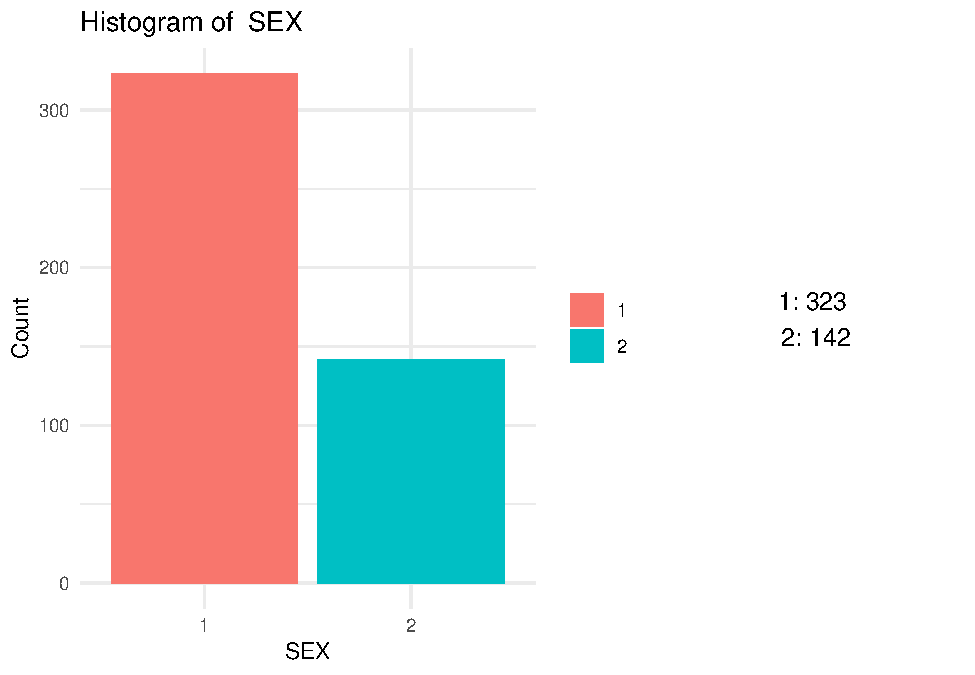
\includegraphics{Q3_markdown_files/figure-latex/unnamed-chunk-5-1.pdf}

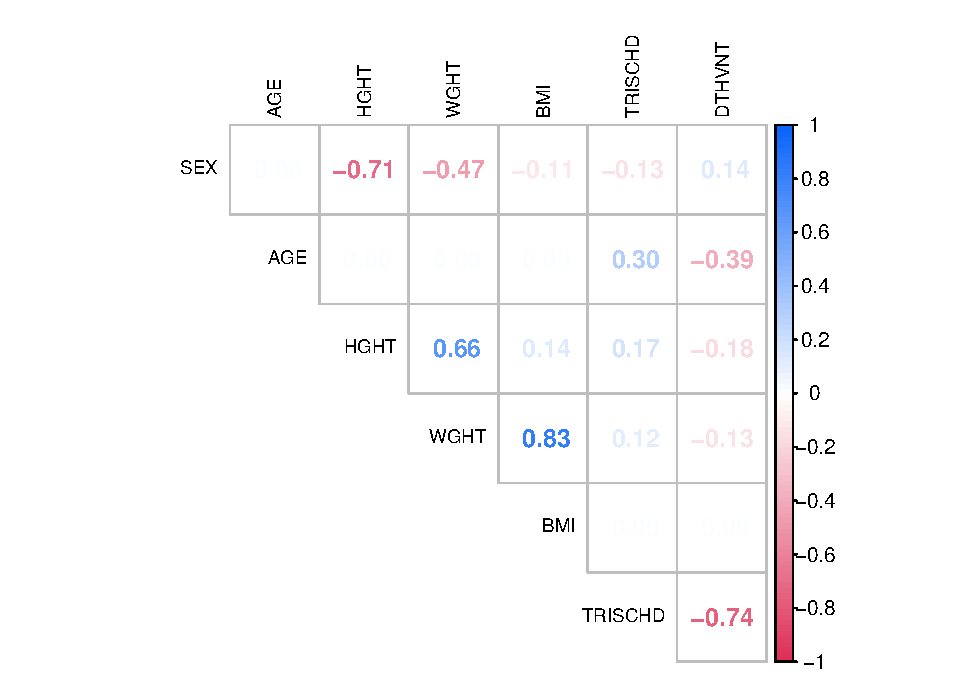
\includegraphics{Q3_markdown_files/figure-latex/unnamed-chunk-6-1.pdf}
\includegraphics{Q3_markdown_files/figure-latex/unnamed-chunk-6-2.pdf}

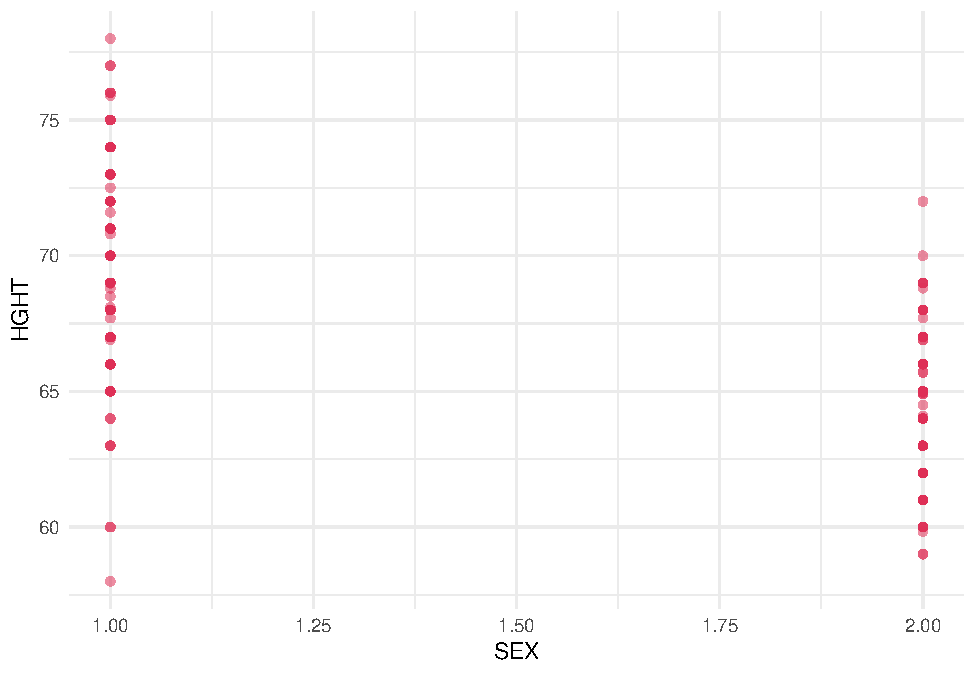
\includegraphics{Q3_markdown_files/figure-latex/unnamed-chunk-7-1.pdf}
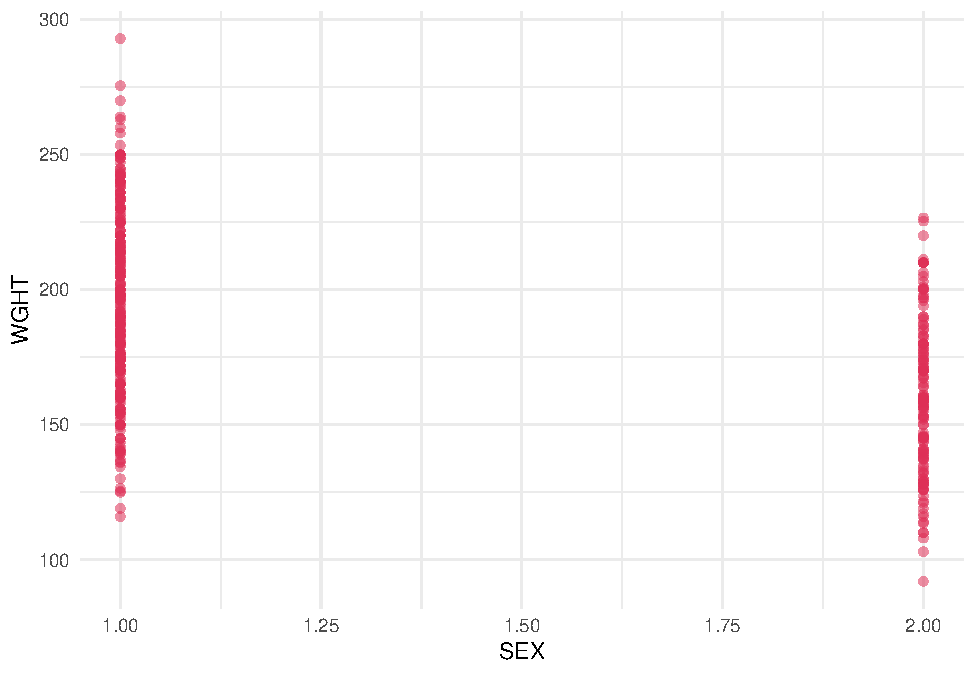
\includegraphics{Q3_markdown_files/figure-latex/unnamed-chunk-7-2.pdf}

Filtering steps:

\begin{verbatim}
## [1] 16110
\end{verbatim}

\begin{verbatim}
## Warning: Setting row names on a tibble is deprecated.
## Setting row names on a tibble is deprecated.
\end{verbatim}

\begin{verbatim}
## [1] TRUE
\end{verbatim}

\begin{verbatim}
## [1] TRUE
\end{verbatim}

\begin{verbatim}
## converting counts to integer mode
\end{verbatim}

\begin{verbatim}
##   the design formula contains one or more numeric variables with integer values,
##   specifying a model with increasing fold change for higher values.
##   did you mean for this to be a factor? if so, first convert
##   this variable to a factor using the factor() function
\end{verbatim}

\begin{verbatim}
##   the design formula contains one or more numeric variables that have mean or
##   standard deviation larger than 5 (an arbitrary threshold to trigger this message).
##   Including numeric variables with large mean can induce collinearity with the intercept.
##   Users should center and scale numeric variables in the design to improve GLM convergence.
\end{verbatim}

\begin{verbatim}
## estimating size factors
\end{verbatim}

\begin{verbatim}
## estimating dispersions
\end{verbatim}

\begin{verbatim}
## gene-wise dispersion estimates
\end{verbatim}

\begin{verbatim}
## mean-dispersion relationship
\end{verbatim}

\begin{verbatim}
## final dispersion estimates
\end{verbatim}

\begin{verbatim}
## fitting model and testing
\end{verbatim}

\begin{verbatim}
## -- replacing outliers and refitting for 54 genes
## -- DESeq argument 'minReplicatesForReplace' = 7 
## -- original counts are preserved in counts(dds)
\end{verbatim}

\begin{verbatim}
## estimating dispersions
\end{verbatim}

\begin{verbatim}
## fitting model and testing
\end{verbatim}

\hypertarget{select-significant-regulations}{%
\subsubsection{Select significant
regulations}\label{select-significant-regulations}}

\hypertarget{select-up-regulations}{%
\subsubsection{Select up-regulations}\label{select-up-regulations}}

\includegraphics{Q3_markdown_files/figure-latex/unnamed-chunk-15-1.pdf}
\includegraphics{Q3_markdown_files/figure-latex/unnamed-chunk-15-2.pdf}

\hypertarget{order-the-dataframe}{%
\subsubsection{Order the dataframe}\label{order-the-dataframe}}

Objective is to have the max values at the top

\begin{verbatim}
## [1] 0.002135431
\end{verbatim}

The ten most significant up-regulated genes are:

\begin{verbatim}
## log2 fold change (MLE): Mophological.cluster.G4 0 
## Wald test p-value: Mophological.cluster.G4 0 
## DataFrame with 10 rows and 6 columns
##                      baseMean log2FoldChange       lfcSE      stat      pvalue
##                     <numeric>      <numeric>   <numeric> <numeric>   <numeric>
## ENSG00000099194.5   3399.6094     0.00213543 0.000193528  11.03420 2.61368e-28
## ENSG00000151365.2    244.4178     0.00198277 0.000187139  10.59517 3.13769e-26
## ENSG00000184811.3    187.0661     0.00174788 0.000173482  10.07529 7.10505e-24
## ENSG00000167588.12   449.1888     0.00159944 0.000152775  10.46923 1.19613e-25
## ENSG00000138207.13   307.0476     0.00143694 0.000155522   9.23941 2.47863e-20
## ENSG00000198695.2  46284.2249     0.00142131 0.000107181  13.26082 3.90624e-40
## ENSG00000140961.12  1158.8132     0.00139424 0.000109770  12.70143 5.80575e-37
## ENSG00000267653.1     92.9383     0.00138503 0.000154817   8.94626 3.67744e-19
## ENSG00000171658.8    247.1142     0.00131334 0.000123903  10.59979 2.98635e-26
## ENSG00000157150.4   1540.0213     0.00129189 0.000113408  11.39160 4.60455e-30
##                           padj
##                      <numeric>
## ENSG00000099194.5  7.12205e-26
## ENSG00000151365.2  5.48312e-24
## ENSG00000184811.3  8.15913e-22
## ENSG00000167588.12 1.79722e-23
## ENSG00000138207.13 1.37886e-18
## ENSG00000198695.2  3.14003e-36
## ENSG00000140961.12 1.55565e-33
## ENSG00000267653.1  1.62871e-17
## ENSG00000171658.8  5.33462e-24
## ENSG00000157150.4  1.68244e-27
\end{verbatim}

\begin{verbatim}
## 
## out of 16110 with nonzero total read count
## adjusted p-value < 0.1
## LFC > 0 (up)       : 4833, 30%
## LFC < 0 (down)     : 6085, 38%
## outliers [1]       : 33, 0.2%
## low counts [2]     : 0, 0%
## (mean count < 42)
## [1] see 'cooksCutoff' argument of ?results
## [2] see 'independentFiltering' argument of ?results
\end{verbatim}

\begin{verbatim}
## 
## out of 4481 with nonzero total read count
## adjusted p-value < 0.1
## LFC > 0 (up)       : 4481, 100%
## LFC < 0 (down)     : 0, 0%
## outliers [1]       : 0, 0%
## low counts [2]     : 0, 0%
## (mean count < 42)
## [1] see 'cooksCutoff' argument of ?results
## [2] see 'independentFiltering' argument of ?results
\end{verbatim}

\includegraphics{Q3_markdown_files/figure-latex/unnamed-chunk-18-1.pdf}
\includegraphics{Q3_markdown_files/figure-latex/unnamed-chunk-18-2.pdf}

\end{document}
